\documentclass[12pt]{article}
\usepackage[utf8]{inputenc}
\usepackage{amsmath}
\usepackage[T1]{fontenc}

\title{ECE 3413 Lab 08\\*DC Motor Model for Open-loop Control in MATLAB Simulink}
\author{Leomar Dur\'an}
\date{${12}^{\text{th}}$ April 2023}

\usepackage[natbib,style=apa6]{biblatex}
\addbibresource{main.bib}
\defbibheading{bibliography}[\refname]{%
  \section*{\centering #1}%
}%

\usepackage{hyperref}

\usepackage{cancel}
\usepackage[per-mode=symbol]{siunitx}
\newcommand*\siexpr[2][]{\SI[parse-numbers=false,#1]{#2}}%
\usepackage{xfrac}
\usepackage{amssymb}
\newcommand*\transpose{\mathsf{T}}

\usepackage{mathtools}%
\DeclarePairedDelimiter\brao()%
\DeclarePairedDelimiter\brac[]%
\DeclarePairedDelimiter\braco[)%
\DeclarePairedDelimiter\braoo][%
\DeclarePairedDelimiter\Brac\{\}%
\DeclarePairedDelimiter\abs||
\DeclarePairedDelimiter\norm\lVert\rVert%
\DeclarePairedDelimiter\piecefn\{.
\DeclarePairedDelimiter\evalat.|

\usepackage{lib/nonfloatenvirons}
\usepackage{booktabs}
\newcommand\ra[1]{\renewcommand*\arraystretch{#1}}
\ra{1.25}

\usepackage{minted}
\newcommand\matlab{matlab}

\usepackage{adjustbox}
\newcommand{\setprime}[2][1]{%
    {#2}^{%
        \raisebox{1pt}{%
            \scalebox{0.5}{%
                \itshape\sffamily\uppercase%
                \expandafter{%
                    \romannumeral#1%
                }%
            }%
        }
    }%
}%
\newcommand*\mcadj[7]%
% {#columns}{col spec}{rotation}{adjust spec}
% {before rotated text}{rotated text}{after rotated text}
{%
    \multicolumn{#1}{#2}{%
        \rlap{%
            #5\adjustbox{rotate=#3,#4}{#6}~#7%
        }%
    }%
}

\usepackage{pdfpages}
\usepackage{standalone}
\usepackage{matlab}

\usepackage[skip=\baselineskip,indent=0pt]{parskip}
\setlength\parindent{0pt}

\usepackage[shortlabels]{enumitem}

\def\hr{{\par\noindent\rule{\textwidth}{0.4pt}}}

\begin{document}

\maketitle
\newpage

\section{Introduction}

This is a two week lab.
Included are both week \texttt\#01 and week \texttt\#02.

The purpose of this lab in week 01 is to analyze a transfer function
and a set of modifications to that transfer function,
whether that be scaling the components of the poles, the natural frequency or adding poles.

This allows us to form relations between these parameters and the characteristics that we expect from a transfer function such as the transient response.

Not only can we estimate the effects that a modification will have on a transfer function, but we can use these relations to find new transfer functions just as one would pick components to have specific effects on a circuit.

In week 02, we also explore the damping of systems and feedback.

\section{Procedure}\label{sec:procedure}

\subsection{Task 0 -- Modeling the DC Motor}\label{ssc:dc motor model}

In this lab, we simulate a DC motor according to the system on page~\pageref{pdf:dc motor model}.
The parameters for this are in the script in \nameref{app} subsection~\ref{sap:default params}.

The motor uses integration in the Laplace domain.
Thus, the integrator system used is merely as shown on page~\pageref{pdf:integrators}.

The DC motor is placed in a simple IPO system as the professor to analyze the motor.
Additionally, we have added a second integrator and a modulus channel to wrap the output around $\braco{0, 2\pi}$.
This produces the angular position (or angle in radians).

The motor can be mathematically described using the model
\begin{equation}
    \brac*{
        \begin{matrix}
            J\ddot\theta\brao*t \\* L\dot{I}\brao*t
        \end{matrix}
    } =
    \brac*{
        \begin{matrix}
            K_t & 0 & -b \\*
            -R & 1 & -K_e \\*
        \end{matrix}
    }\brac*{
        \begin{matrix}
            I \\* V \\* \dot\theta\brao*t
        \end{matrix}
    }.
\end{equation}

\includepdf[pages=2,landscape=true,pagecommand=\label{pdf:dc motor model}]{drawings/lab08_openloop_control_slx.pdf}
\includepdf[pages=3,landscape=true,pagecommand=\label{pdf:integrators}]{drawings/lab08_openloop_control_slx.pdf}
\includepdf[pages=1,landscape=true,pagecommand=\label{pdf:dc motor system}]{drawings/lab08_openloop_control_slx.pdf}

\subsection{Task 1 -- Varying the gains}

We plotted the result of modeling the DC motor with the gains given in \eqref{eq:gains}, representing both the armature torque constant and the back EMF from the motor.

\begin{equation}\label{eq:gains}
    K \in \Brac*{\begin{matrix}.01, & .02, & .3, & .4, & 1, & 2\end{matrix}}.
\end{equation}

We automated this process by using the script in \nameref{app} subsection~\ref{sap:vary gains}.

\subsection{Task 2 -- Plotting the angular velocity response}

After this, we see the effect of the default parameters on the motor, using the script in \nameref{app} subsection~\ref{sap:plotting angular velocity}.

\subsection{Tasks 03(a), 4 -- Varying the moment of inertia of the motor}

We plotted the result of modeling the DC motor with the moments of inertia given in \eqref{eq:moments of inertia}.

\begin{equation}\label{eq:moments of inertia}
    K \in \Brac*{\begin{matrix}.1, & 1, & 5\end{matrix}}.
\end{equation}

We automated this process by using the script in \nameref{app} subsection~\ref{sap:vary moment of inertia}.

\subsection{Tasks 03(b), 4 -- Varying the damping ratio of the mechanical system}

We plotted the result of modeling the DC motor with the damping ratios of the mechanical systems in \eqref{eq:damping ratios}.

\begin{equation}\label{eq:damping ratios}
    K \in \Brac*{\begin{matrix}.01 & .1 & .2\end{matrix}}.
\end{equation}

We automated this process by using the script in \nameref{app} subsection~\ref{sap:vary damping ratio}.


\subsection{Task 05 -- Parameters to repeat the angle period}

Finally, we use the scope for the angular position mentioned in subsection~\ref{ssc:dc motor model}.

The parameters for this are in the script in \nameref{app} subsection~\ref{sap:repeat angle params}. 
Rather than the default time of $\SI{10.0}\second$,
we use $\SI{100.0}\second$
to show the angle period repeating.

\section{Results}

\subsection{Task 1 -- Varying the gains}

\begin{figure}
    \centering
    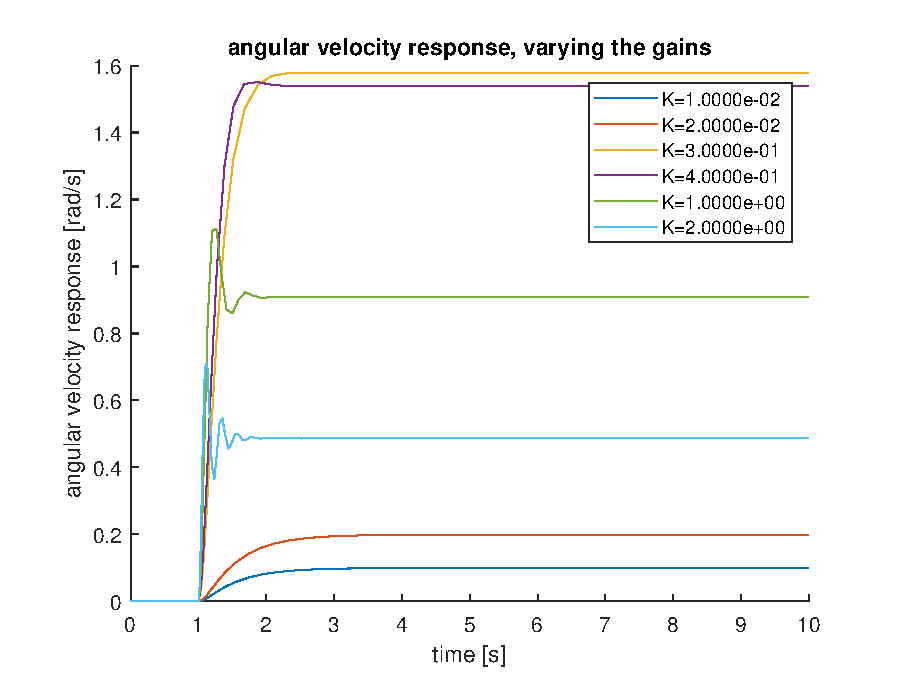
\includegraphics[width=\linewidth]{img/task01_varying_gains.eps}
    \caption{Effect of gains on the angular velocity response.}
    \label{fig:gains on angular velocity}
\end{figure}

\subsection{Task 2 -- Plotting the angular velocity response}

\begin{figure}
    \centering
    \includegraphics[width=\linewidth]{img/task02_plot_angular_velocity.eps}
    \caption{Plot of the angular velocity response.}
    \label{fig:plot of angular velocity}
\end{figure}

\subsection{Tasks 03(a), 4 -- Varying the moment of inertia of the motor}

\begin{figure}
    \centering
    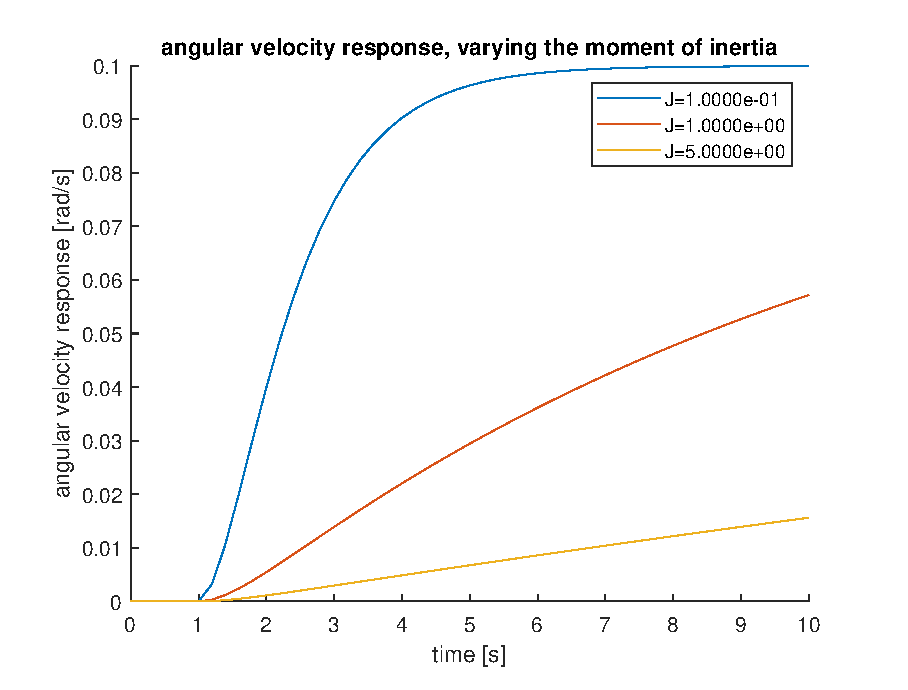
\includegraphics[width=\linewidth]{img/task03a_varying_moment_of_inertia.eps}
    \caption{Effect of the moment of inertia on the angular velocity response.}
    \label{fig:moment of inertia on angular velocity}
\end{figure}

\subsection{Tasks 03(b), 4 -- Varying the damping ratio of the mechanical system}

\begin{figure}
    \centering
    \includegraphics[width=\linewidth]{img/task03b_varying_mechanical_sys_damping_ratio.eps}
    \caption{Effect of the damping ratio of the mechanical system on the angular velocity response.}
    \label{fig:mechanical system damping ratio on angular velocity}
\end{figure}

\subsection{Task 05 -- The angular position vs time}

\begin{figure}
    \centering
    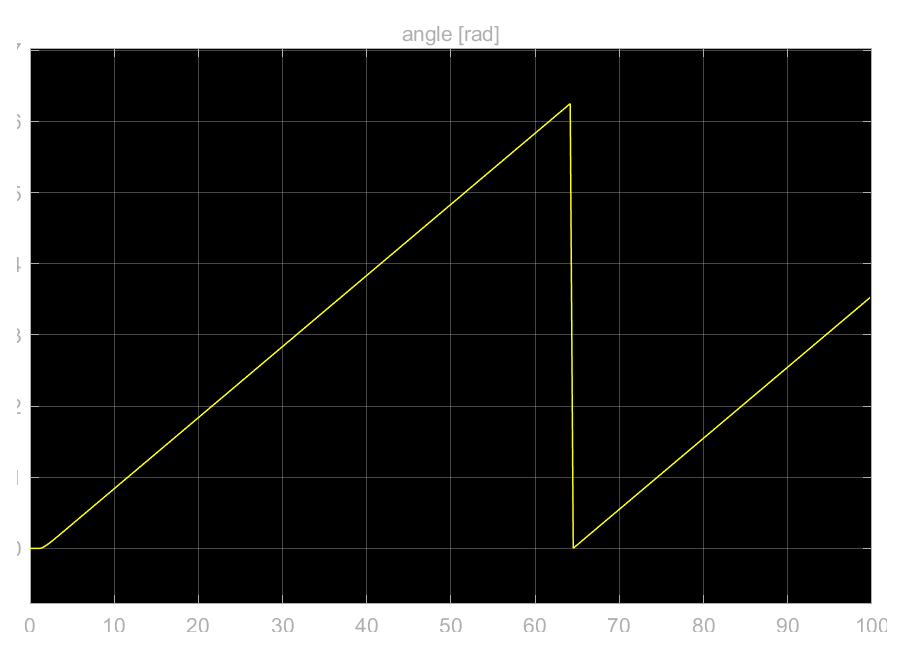
\includegraphics[width=\linewidth]{img/task05_angular_position.eps}
    \caption{The angular position of the motor.}
    \label{fig:angular position of motor}
\end{figure}
\section{Discussion}

\paragraph{For week 01}

In this lab, we learned that manipulating the real and imaginary parts of the poles will effect their $x$- and $y$-components respectively, and that manipulating the natural frequency will effect the poles' magnitudes.

Regarding this, I learned that graphing in the polar co\"ordinate system is not as well supported by Matlab as the Cartesian co\"ordinate system.
There is a \mintinline\matlab{polarplot} function.
However it does not support multiple plots and cannot be combined with a plot in Cartesian.
Because of this, going forward, I will use \mintinline\matlab{pzmap} instead;
and if I need to use the more primitive facilities of polar co\"ordinate system,
then I will have to prefer to find an alternative system such as Python.


This lab also gave us the opportunity to test the hypothesis that a positive real pole will always be result in an unstable transfer function, whereas a transfer function where all poles only have non-positive real part will be stable.
Additionally, we have learned that the poles with real part closest to $0$ dominate.
It is also a good time to remember that a pole that has $5\times$ the real part $-\zeta\omega_n$ of another pole
will have very little significant effect in comparison.
This former pole is $5\tau$ away from the latter pole.

Now we can see that the rise time has no direct relationship with the roots or the natural frequency.
Because of this, we had to use the Matlab equation solver to find the appropriate times at $\SI{10}\percent$ and $\SI{90}\percent$ final output,
and from this calculate the rise times.

From Table~\ref{tab:rise time changing poles}, we can confirm no obvious relation for the components of the pole. However, there seems to be a scaling effect to the natural frequency. Let's investigate further.

\begin{figure}
    \centering
    %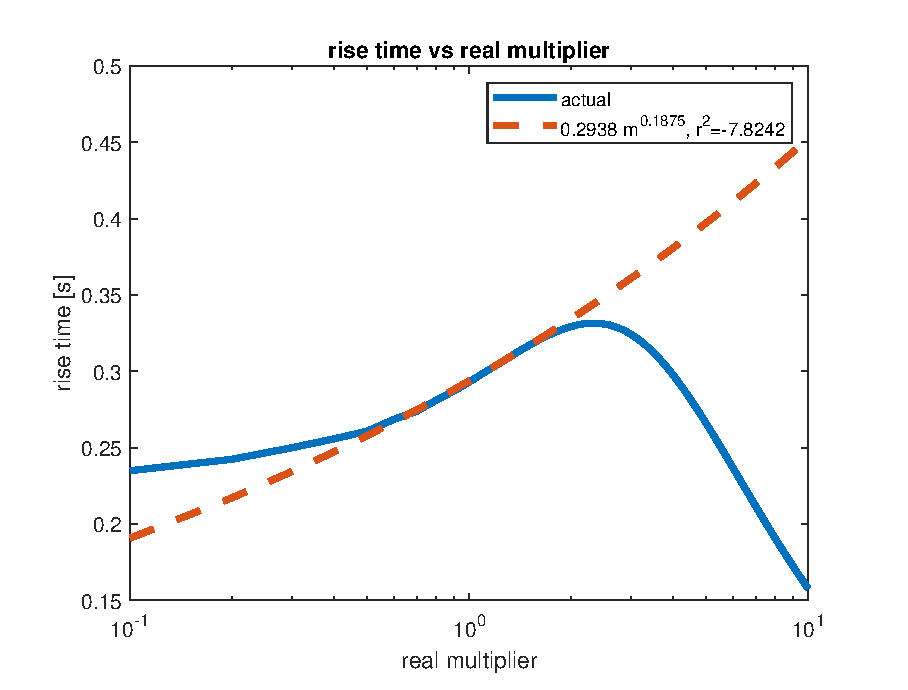
\includegraphics[width=\linewidth]{img/part01_rise_time_vs_real.eps}
    \caption{Plot in a semi-log scale on the $x$-axis
    showing the effect of multiplying the real component of the poles on the rise time and log-log linear regression.}
    \label{fig:rise time vs real}
\end{figure}

The script in Appendix subsection~\ref{sap:rise time vs parameters}
plots the rise time vs the parameters that we have investigated
in a semi-log scale on the $x$-axis
from the reciprocal of the modification to the modification.
(For the imaginary part, this is the reverse because the modification was scaling by $\sfrac12$.)
A log-log linear regression is taken from these, and then the entire plot is scaled by $5$ on each side
to allow for scaling.

This produces Fig.~\ref{fig:rise time vs real}, \ref{fig:rise time vs imag} and \ref{fig:rise time vs wn}.

\paragraph{Note that} since the Matlab equation solver is time expensive and each plot will use $100$ samples, we use the Matlab \mintinline\matlab{stepinfo} function to find the rise time, albeit it does not the bounds of the rise time.

\begin{figure}
    \centering
    %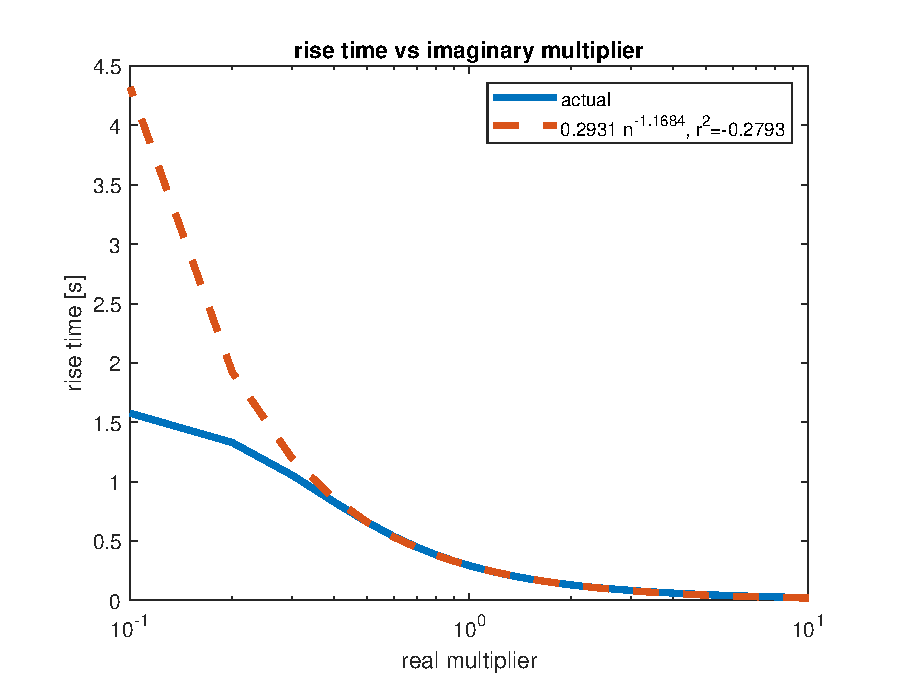
\includegraphics[width=\linewidth]{img/part01_rise_time_vs_imag.eps}
    \caption{Plot in a semi-log scale on the $x$-axis
    showing the effect of multiplying the imaginary component of the poles on the rise time and log-log linear regression.}
    \label{fig:rise time vs imag}
\end{figure}

Now, the coefficients in $\brac{\begin{matrix}0.2938 & 0.2931 & 0.2930\end{matrix}}$ represent the rise time of the original transfer function,
which we found to be \SI{0.292698}\second in sub-subsection~\ref{sss:evaluations}.
These values represent that rise time with deviation $\num{0.00085651}$.

For modifying the real component, the linear regression
(in Fig.~\ref{fig:rise time vs real})
was only successful locally at $\brac{0.3, 2.3}$ with $r^2 = \num{0.956348}$.
Thus, there does not seem to be a relation between the real component and rise time.

\begin{figure}
    \centering
    %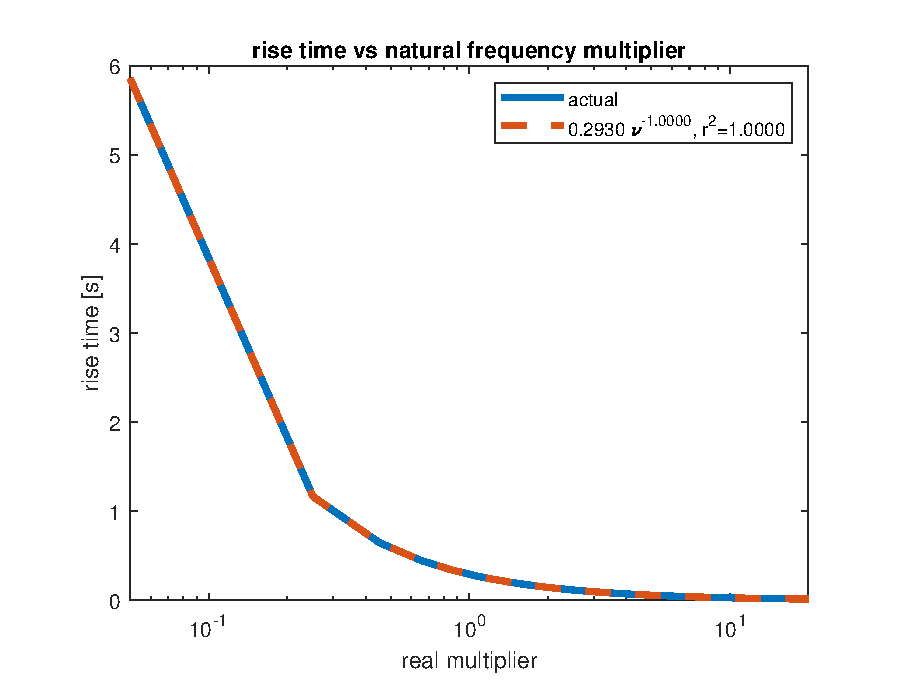
\includegraphics[width=\linewidth]{img/part01_rise_time_vs_wn.eps}
    \caption{Plot in a semi-log scale on the $x$-axis
    showing the effect of multiplying the natural frequency on the rise time and log-log linear regression.}
    \label{fig:rise time vs wn}
\end{figure}

For modifying the imaginary component, the linear regression
(in Fig.~\ref{fig:rise time vs imag})
is much better, having $r^2 = 0.991558$ in $\brac{0.3, 9.8}$.
I predict that after $n = 0.3$, the effect of multiplying the imaginary part by imaginary part of the pole by $n$ will result in a division of the rise time by $n^{1.1684}$.
In fact, taking the original rise time \SI{0.292698}\second and dividing by $\brao*{\sfrac12}^1.1684$ gives $\SI{0.657874}\second$.
The calculated value for the rise time halving the imaginary part of the pole was $\SI{0.658607}\second$.
That's a rate of error of $\SI{-0.111295}\percent$.
Interestingly since the modification was to half the imaginary part, this prediction may not be so useful.

Earlier, we speculated that modifying the natural frequency uniformly moves the range of the rise time.
In Fig.~\ref{fig:rise time vs wn}, we find an $r^2 = 1.0000$ from $\brao{0.05, 19.3955}$.
This appears to be an exact match!
We can predict that multiplying the natural frequency by $\nu$ will result in dividing the rise time by $\nu$.
Now
\begin{equation}
    \frac{T_r}\nu = \frac{\SI{0.292698}\second}4 = \SI{0.0731745}\second \approx \SI{0.073175}\second = \setprime[3]{T}_r
\end{equation}
with a negligible $\SI{-6.83293e-6}{\second^0}$ rate of error.

Moreover, it the natural frequency
scales the time domain
of a transfer function.
Earlier we saw that changing the natural frequency $\setprime\omega_n = \nu\omega_n$ results in
new peak time $\setprime{T}_p = \sfrac{T_p}\nu$ and
new settling time $\setprime{T}_s = \sfrac{T_s}\nu$,
and now we have the relation $\setprime{T}_r = \sfrac{T_r}\nu$
as well as the bounds $\setprime{t}_{.9f} = \sfrac{t_{.9f}}\nu,\ \setprime{t}_{.1f} = \sfrac{t_{.1f}}\nu$
from Table~\ref{tab:rise time changing poles}.
In the case of overshoot, it makes sense that this would not be affected
as overshoot is a characteristic of the range of step response, not the domain.

Thus, we see that generally it is the case that if $c$ is a transfer function with natural frequency $\omega_n$
and $\setprime{c}$ is a transfer function that is almost equivalent, but with natural frequency $\nu\omega_n$,
then
\begin{equation}
    \setprime{c}\brao*{\frac{t}\nu} = c\brao*t.
\end{equation}

\paragraph{For week 02}

We see the effect of the poles on the dampening of the system.

We see that stable systems always have poles in the left half plane, overdamped systems are produced by two complex poles, overdamped systems are produced by two unique real roots, critically damped systems are produced by a double real root and undamped systems are produced by imaginary roots.

The positive feedback always seems to create unstable systems, whereas negative feedback produced similar stable systems that may differ in damping.

\newpage
\printbibliography

\newpage
\appendix
\section{Appendix}\label{app}

\subsection{Task 00 -- Default parameters, Matlab script}\label{sap:default params}
\inputminted{matlab}{src/lab08_task00_default_dc_motor_motor_params.m}

\hr{}

\subsection{Task 01 -- Varying the gains, Matlab script}\label{sap:vary gains}
\inputminted{matlab}{src/lab08_task01_vary_gain.m}

\hr{}

\subsection{Task 02 -- Plotting the angular velocity response, Matlab script}\label{sap:plotting angular velocity}
\inputminted{matlab}{src/lab08_task02_plot_angular_velocity.m}

\hr{}

\subsection{Task 03(a) -- Varying the moment of inertia of the motor, Matlab script}\label{sap:vary moment of inertia}
\inputminted{matlab}{src/lab08_task03a_vary_motor_moment_of_inertia.m}

\subsection{Task 03(b) -- Varying the damping ratio of the mechanical system, Matlab script}\label{sap:vary damping ratio}
\inputminted{matlab}{src/lab08_task03b_vary_mechanical_sys_damping.m}

\subsection{Task 05 -- Parameters to repeat the angle period, Matlab script}\label{sap:repeat angle params}
\inputminted{matlab}{src/lab08_task05_angle_repeat_params.m}

\end{document}
